\chapter{Задание 3. Конденсируй-умножай}

Рассмотрим уравнение конденсатора:
\[
    I = C \frac{dU}{dt}
\]  

со следующими параметрами:
\begin{itemize}
    \item[] \( C = 324 \, \text{мкФ} \)
\end{itemize}

Передаточная функция конденсатора имеет вид:
\[
    W(s) = \frac{U}{I} = \frac{1}{Cs}
\]

Что является идеальным интегрирующим звеном, имеющим передаточную функцию вида:
\[
    W(s) = \frac{K}{s}
\]

Соответственно, коэффициент \( K \) равен:
\[
    K = \frac{1}{C} = 3086.4
\]

\section{Временные характеристики}

Переходная характеристика для интегрирующего звена имеет вид:
\[
    h(t) = K t
\]

Весовая характеристика для интегрирующего звена имеет вид:
\[
    w(t) = K
\]

\begin{figure}[H]
    \centering
    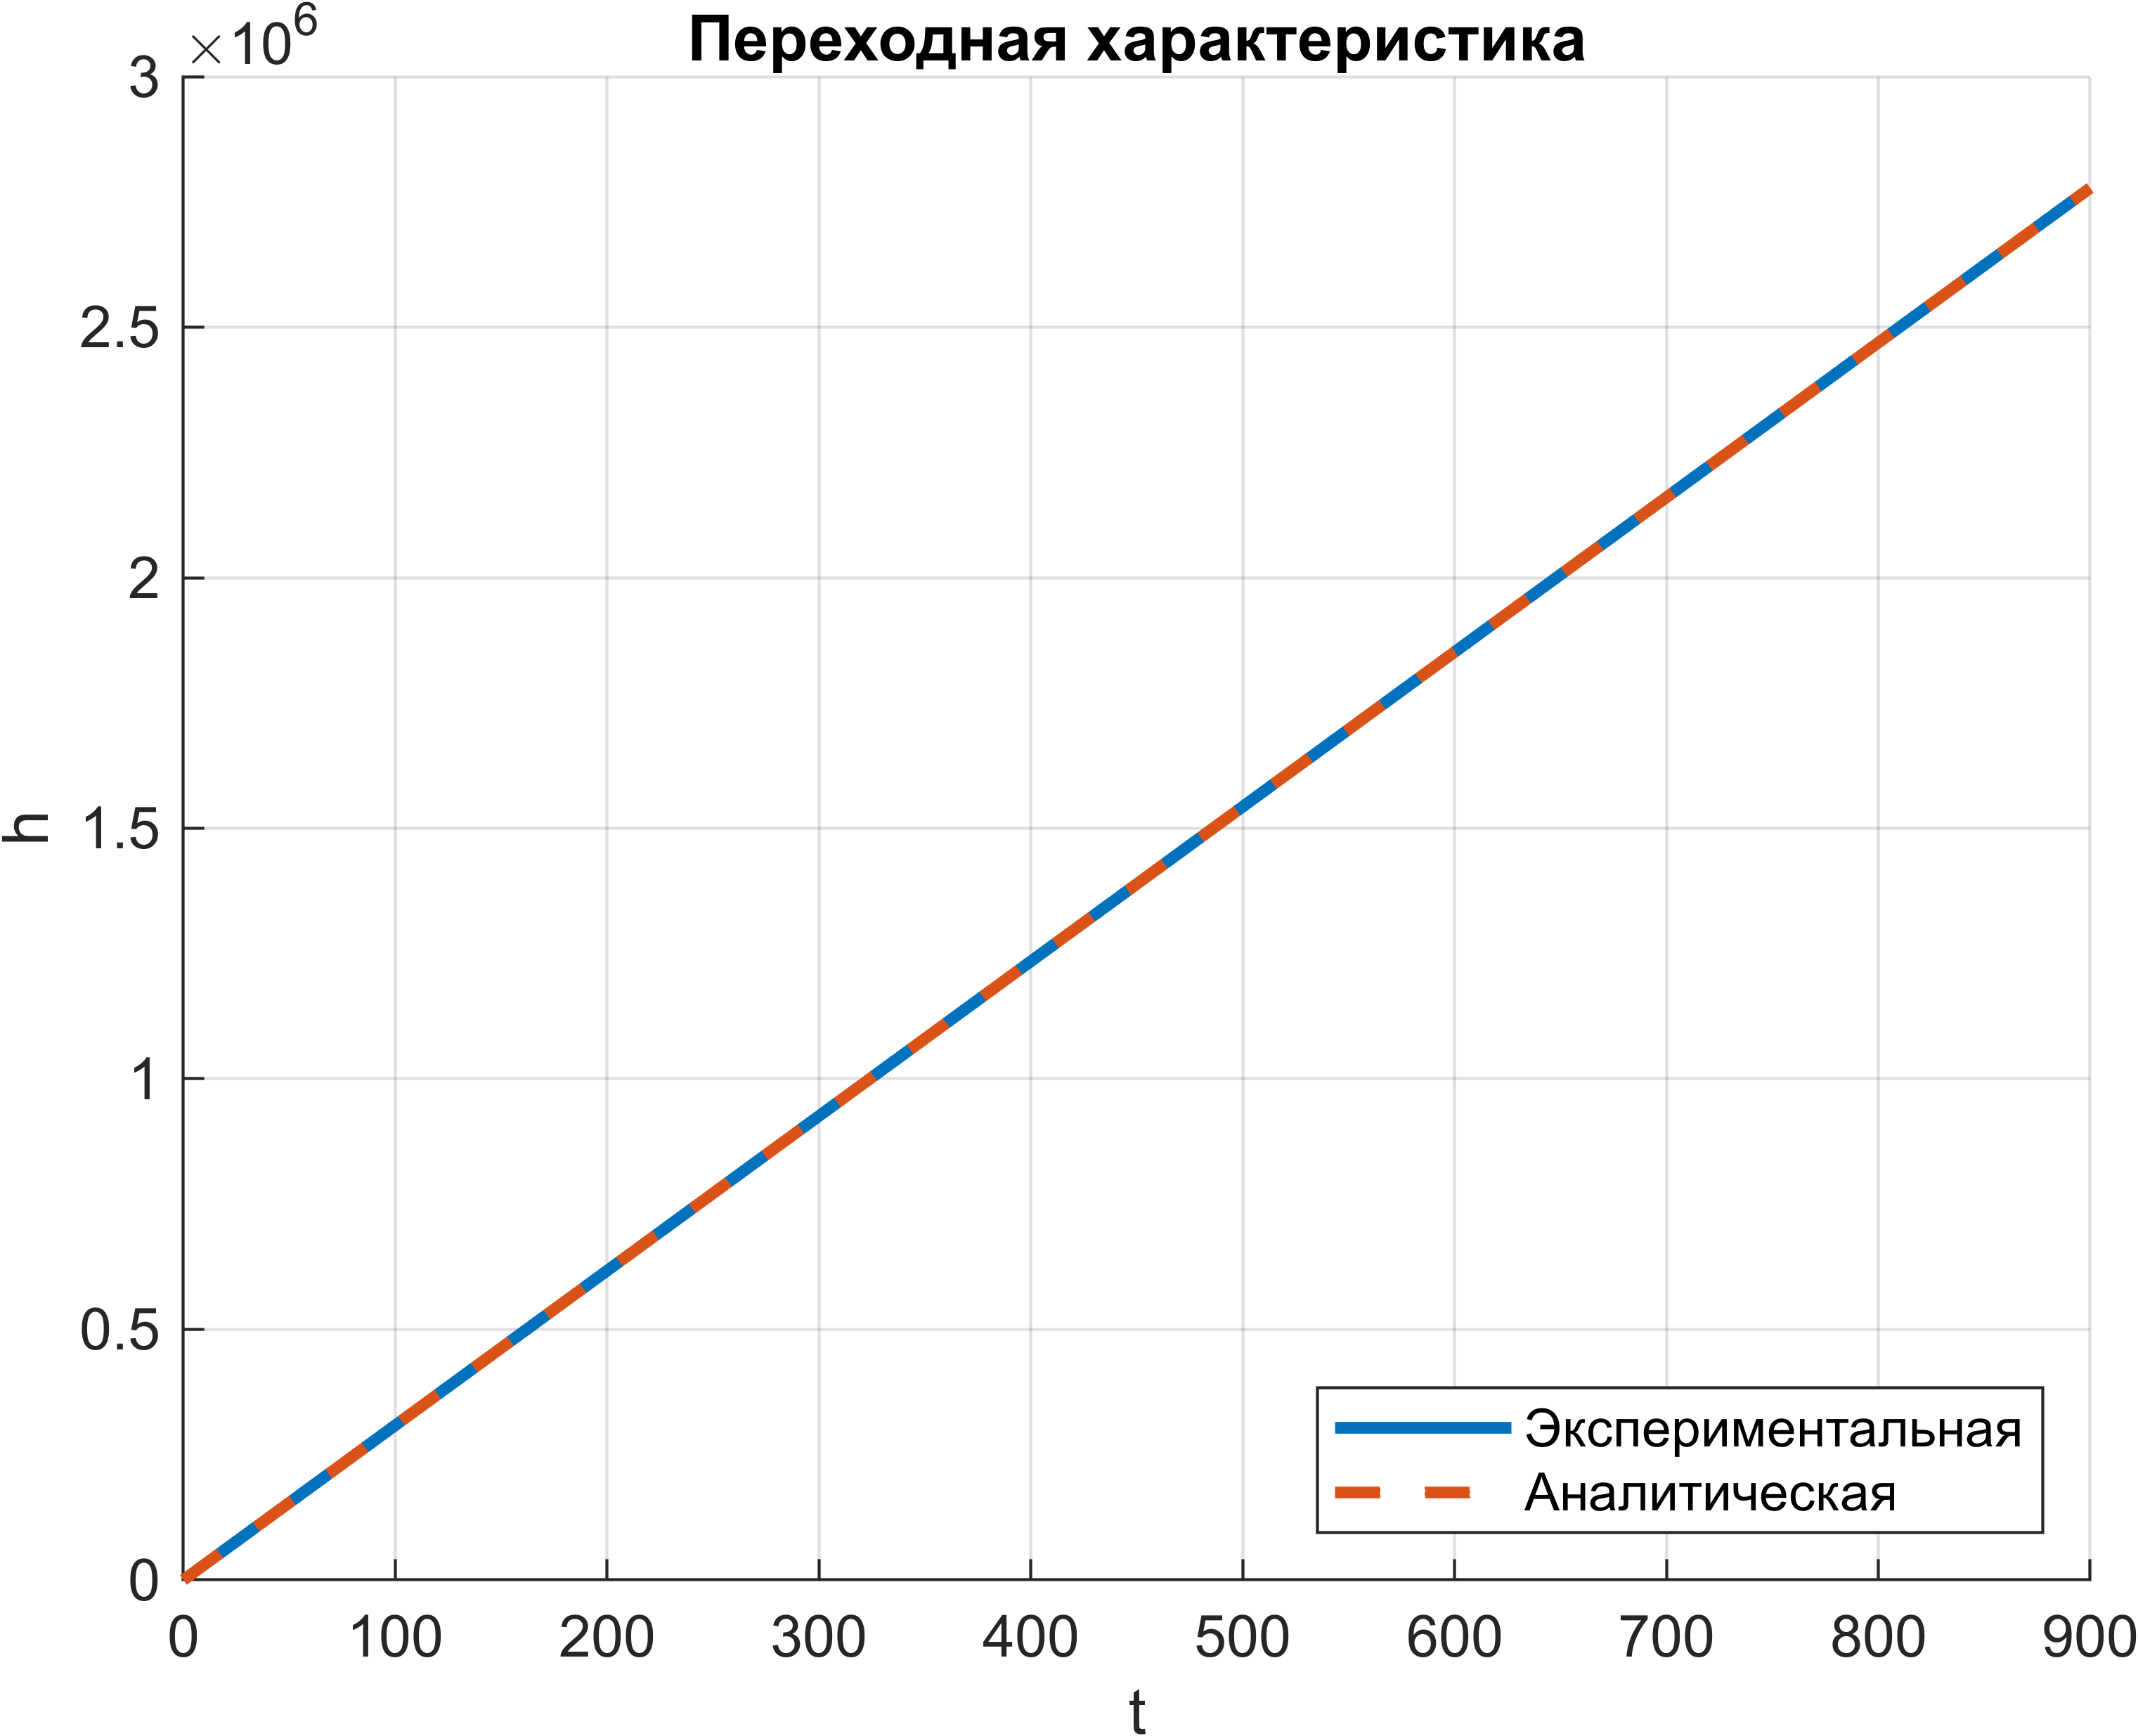
\includegraphics[width=0.75\textwidth, trim={0cm 0cm 0cm 0cm}]{../images/3_1.png}
    \caption{Переходная характеристика конденсатора}
\end{figure}

\begin{figure}[H]
    \centering
    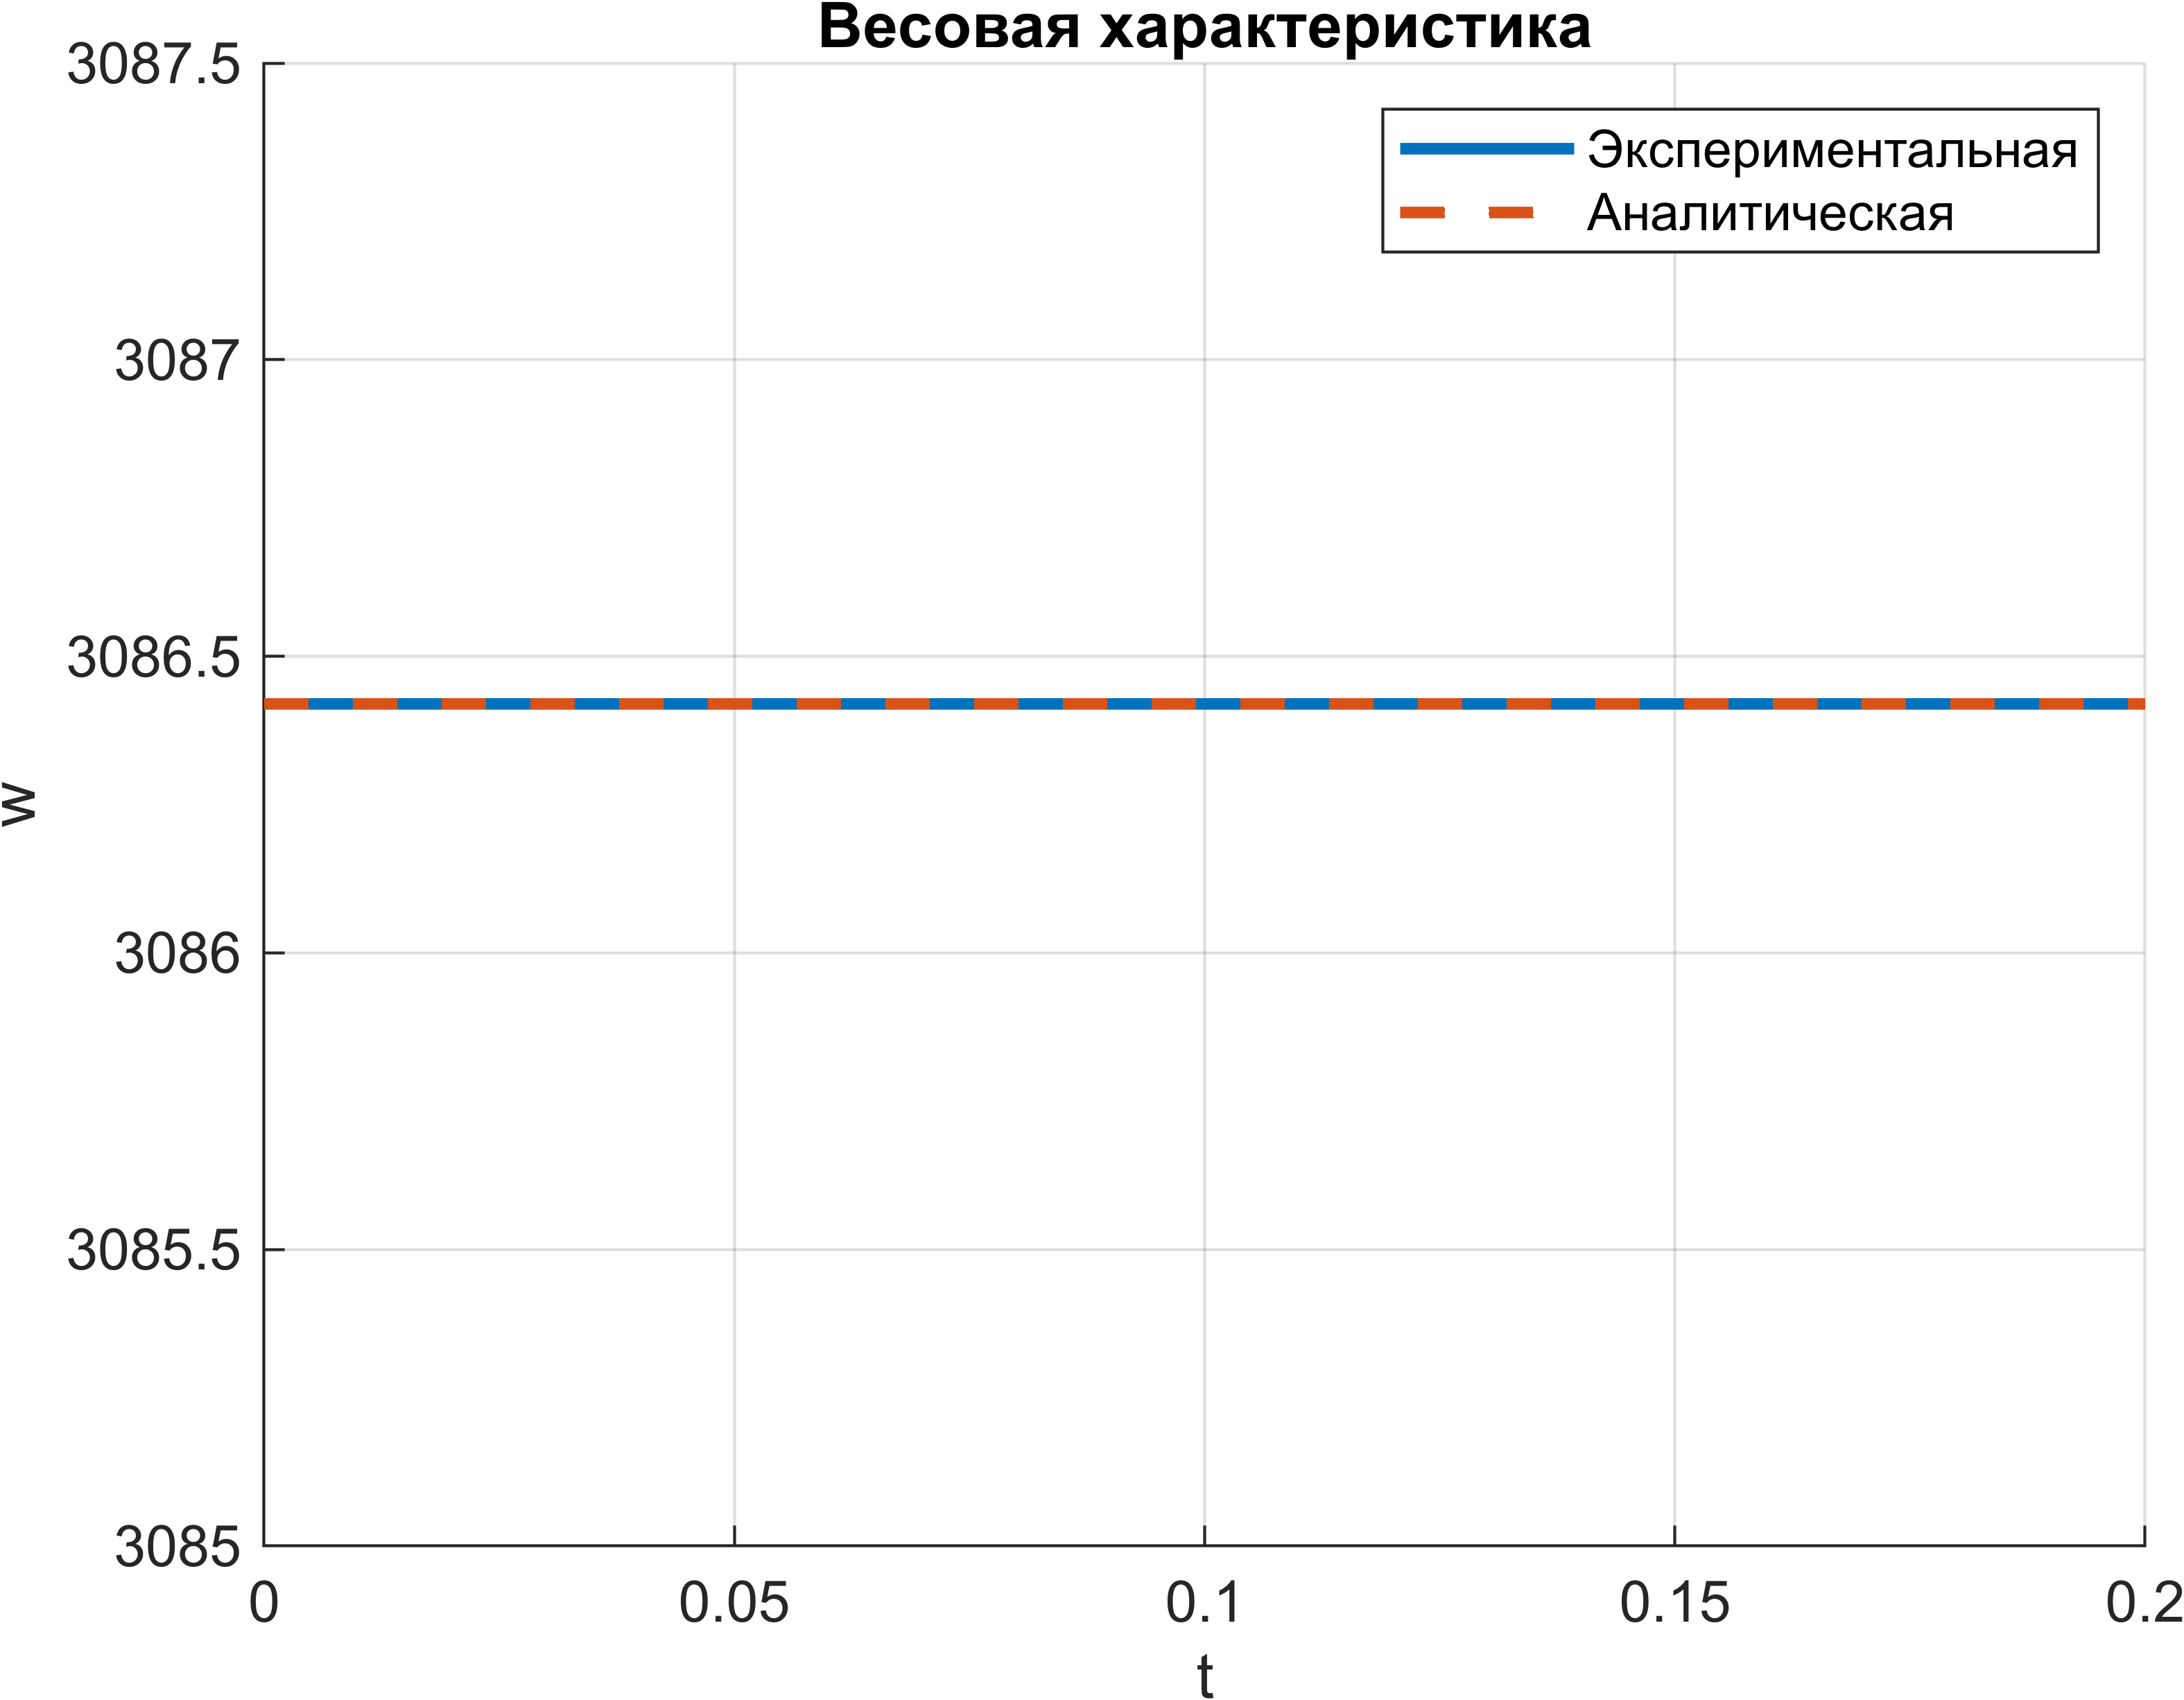
\includegraphics[width=0.75\textwidth, trim={0cm 0cm 0cm 0cm}]{../images/3_2.png}
    \caption{Весовая характеристика конденсатора}
\end{figure}

\section{Частотные характеристики}

Амплитудно-частотная характеристика для интегрирующего звена имеет вид:
\[
    A(\omega) = \frac{K}{\omega}
\]

Логарифмическая амплитудно-частотная характеристика:
\[
    L(\omega) = 20 \lg(K) - 20 \lg(\omega)
\]

Фазо-частотная характеристика для интегрирующего звена имеет вид:
\[
    \phi(\omega) = -\frac{\pi}{2}
\]

\begin{figure}[H]
    \centering
    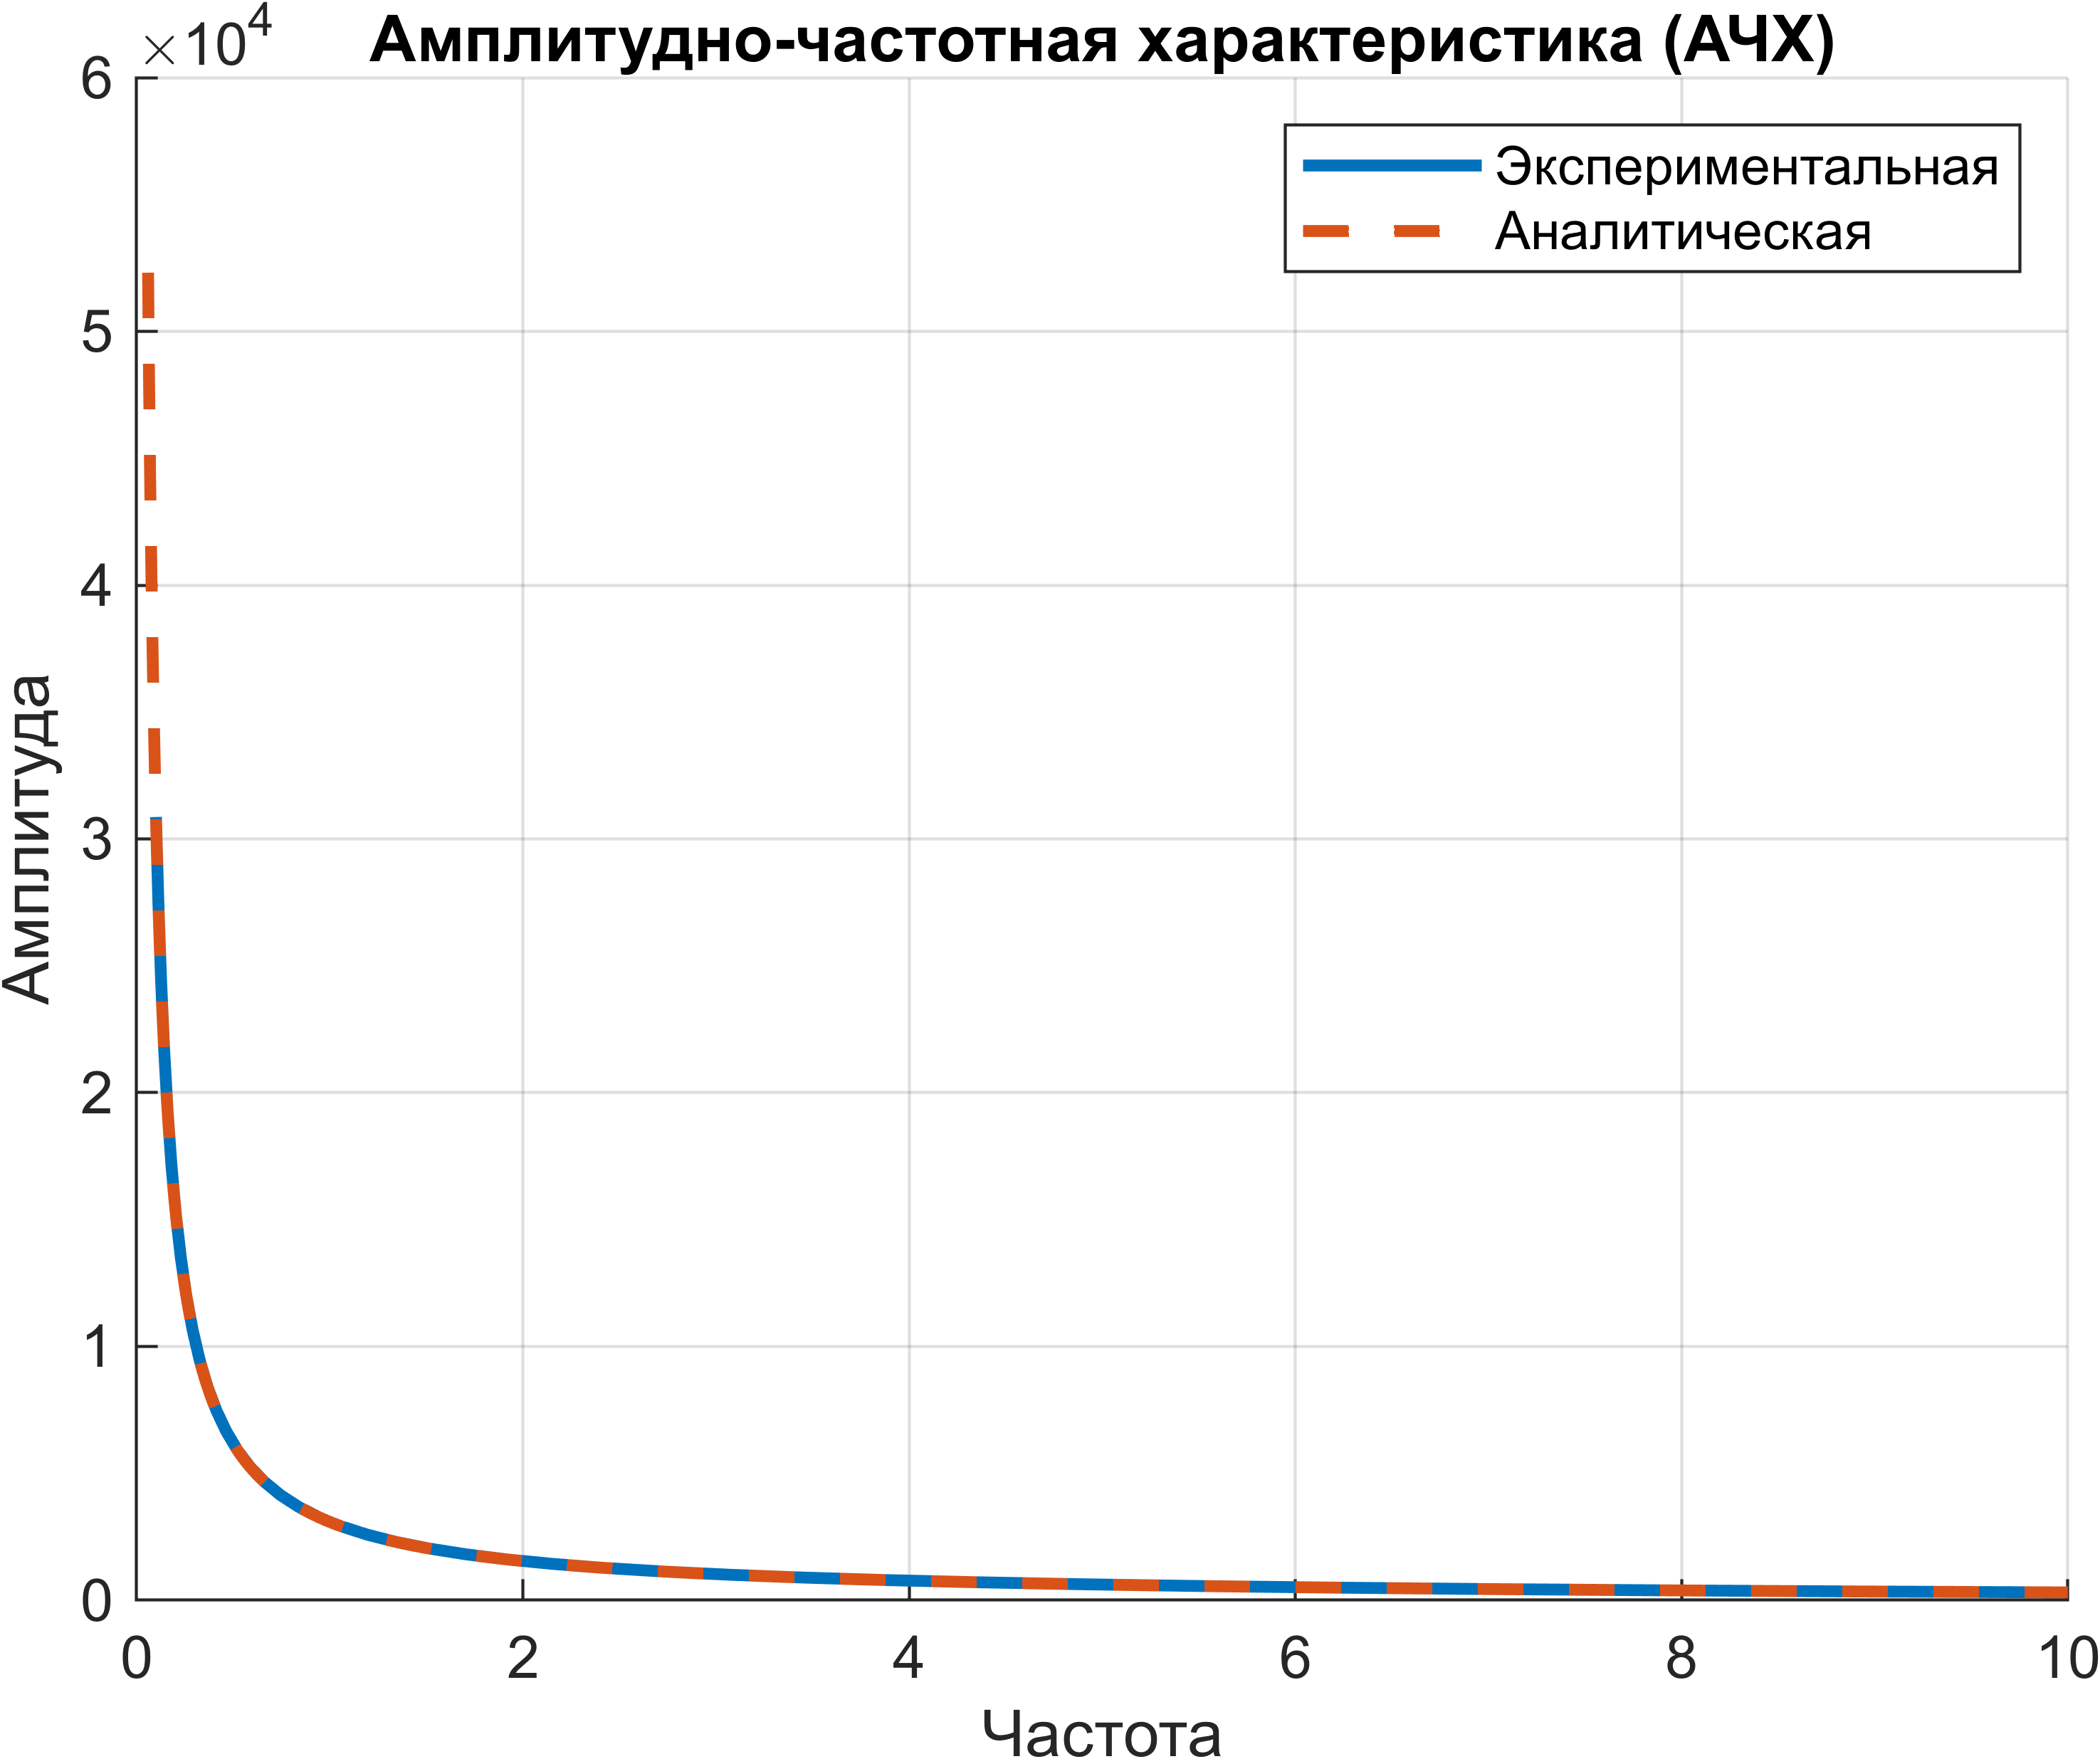
\includegraphics[width=0.75\textwidth, trim={0cm 0cm 0cm 0cm}]{../images/3_3.png}
    \caption{Амплитудно-частотная характеристика конденсатора}
\end{figure}

\begin{figure}[H]
    \centering
    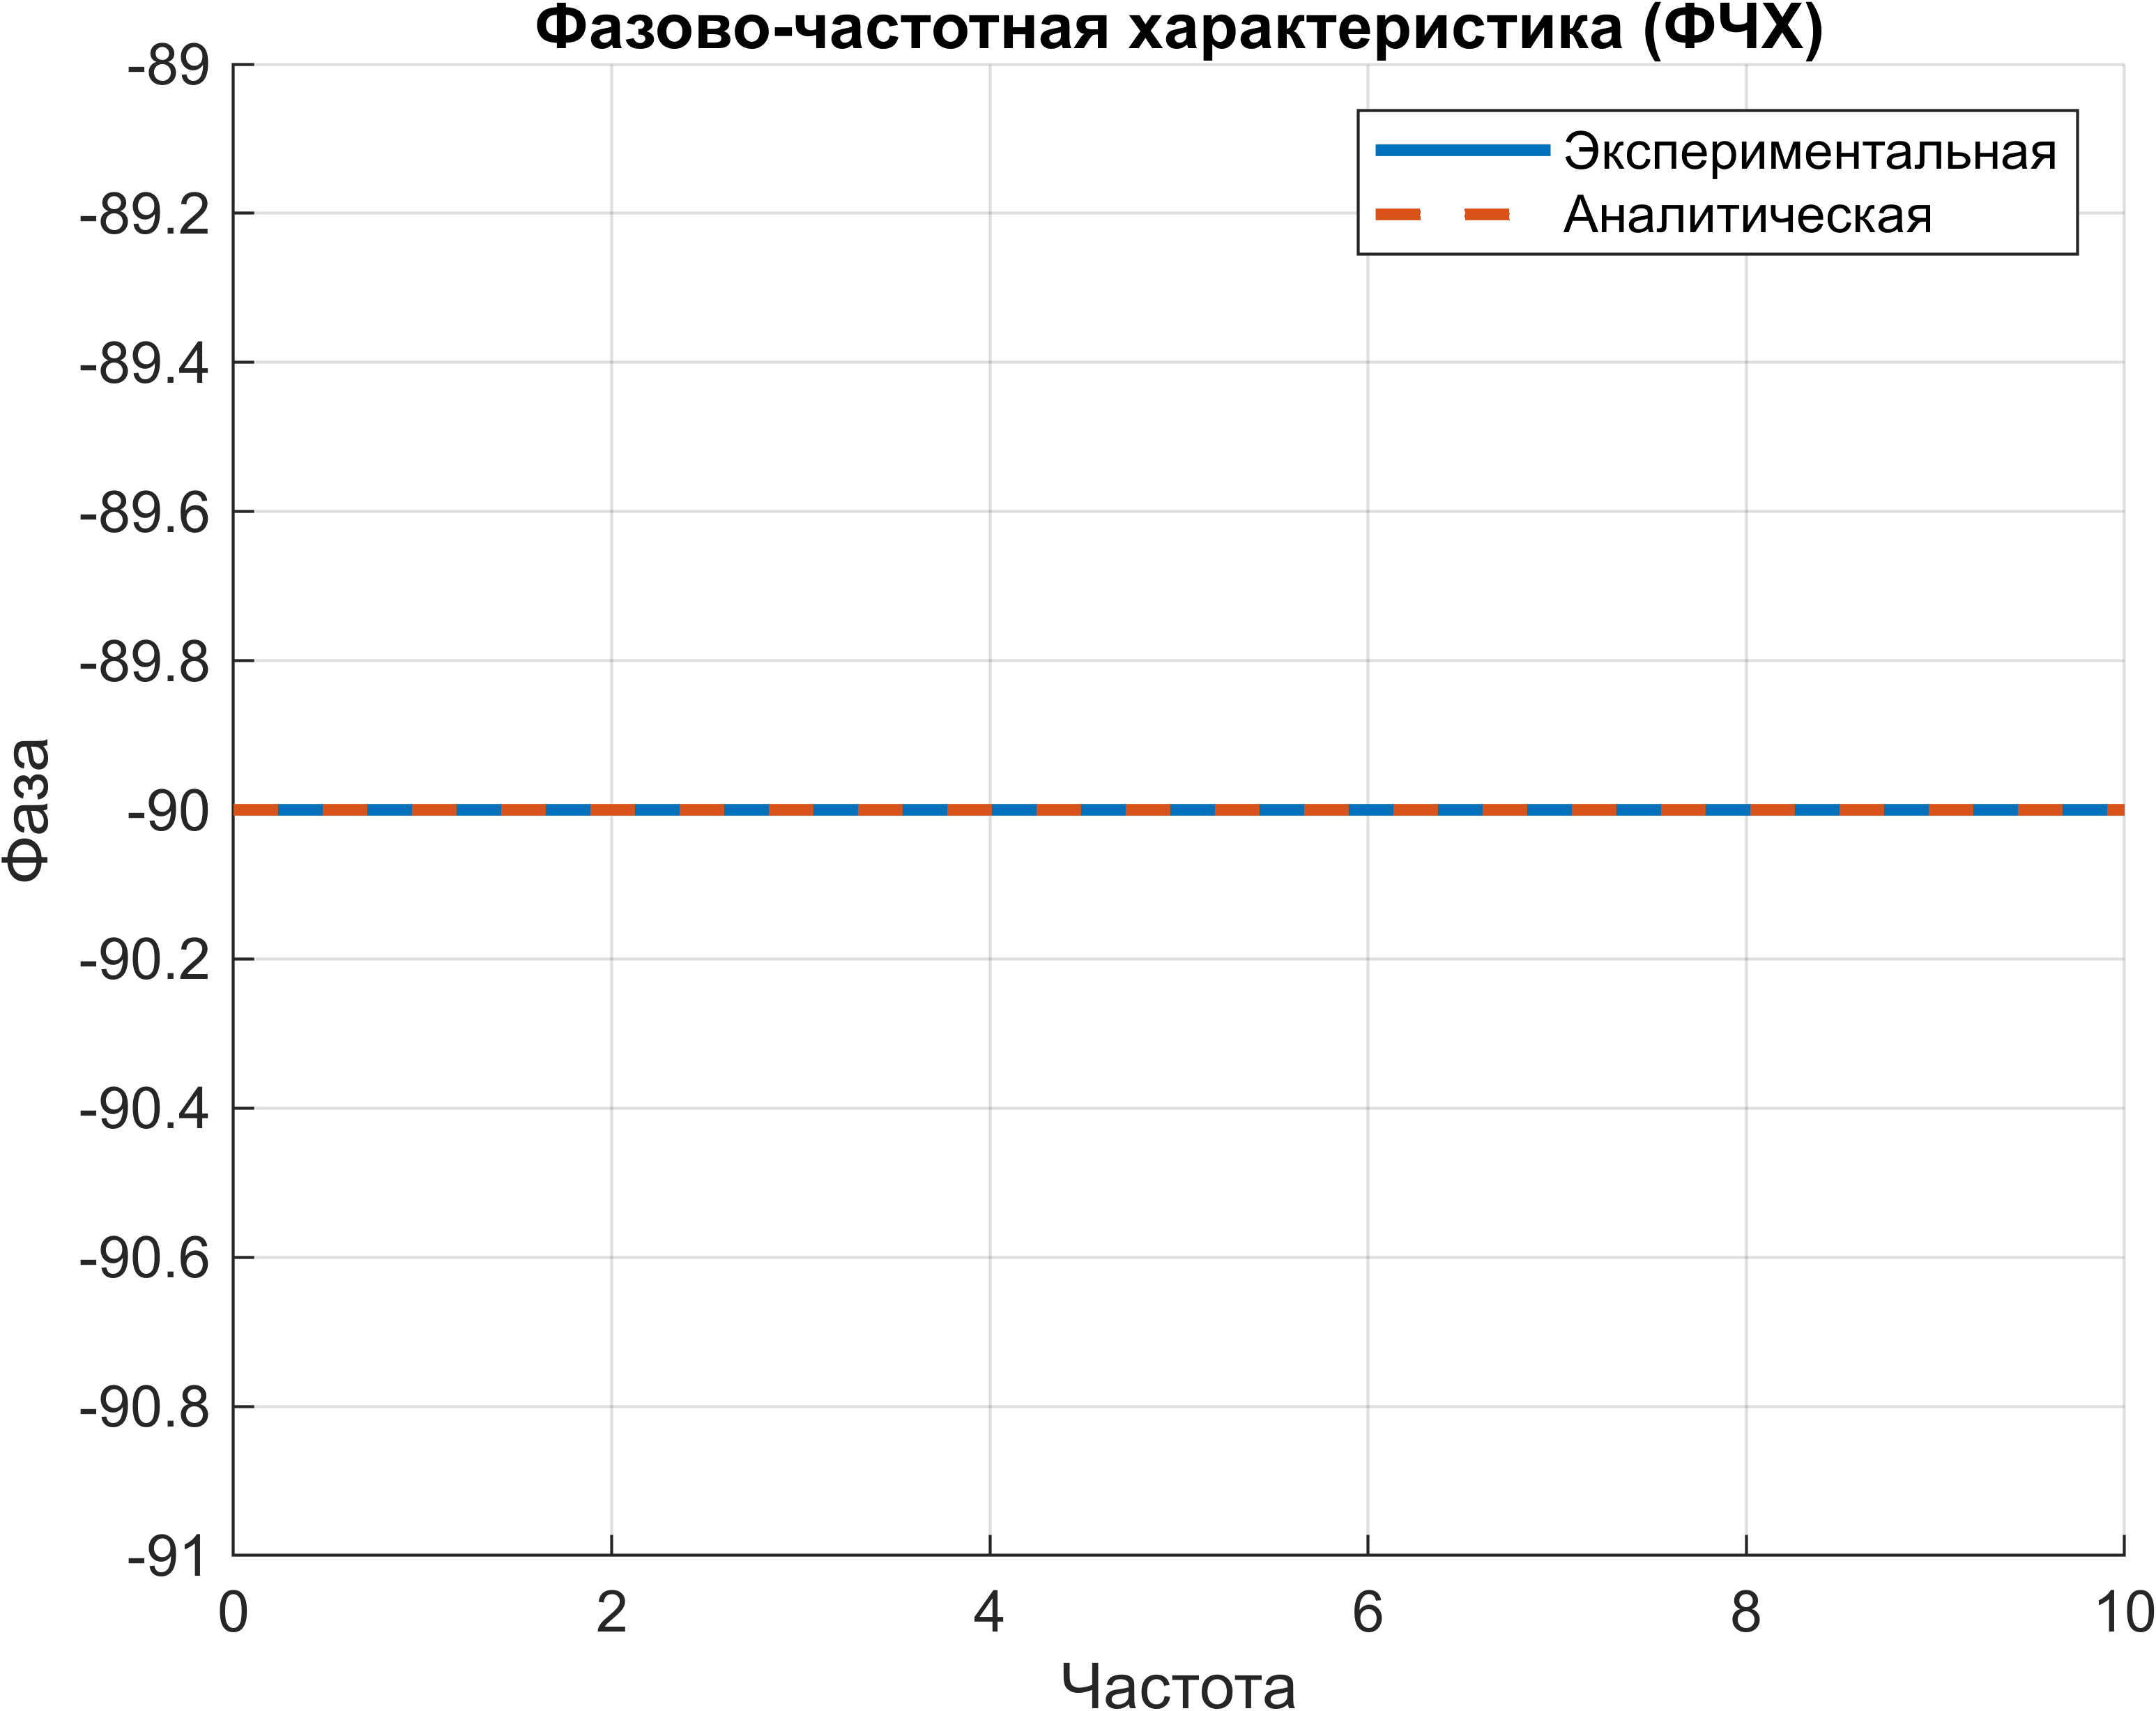
\includegraphics[width=0.75\textwidth, trim={0cm 0cm 0cm 0cm}]{../images/3_4.png}
    \caption{Фазо-частотная характеристика конденсатора}
\end{figure}

\begin{figure}[H]
    \centering
    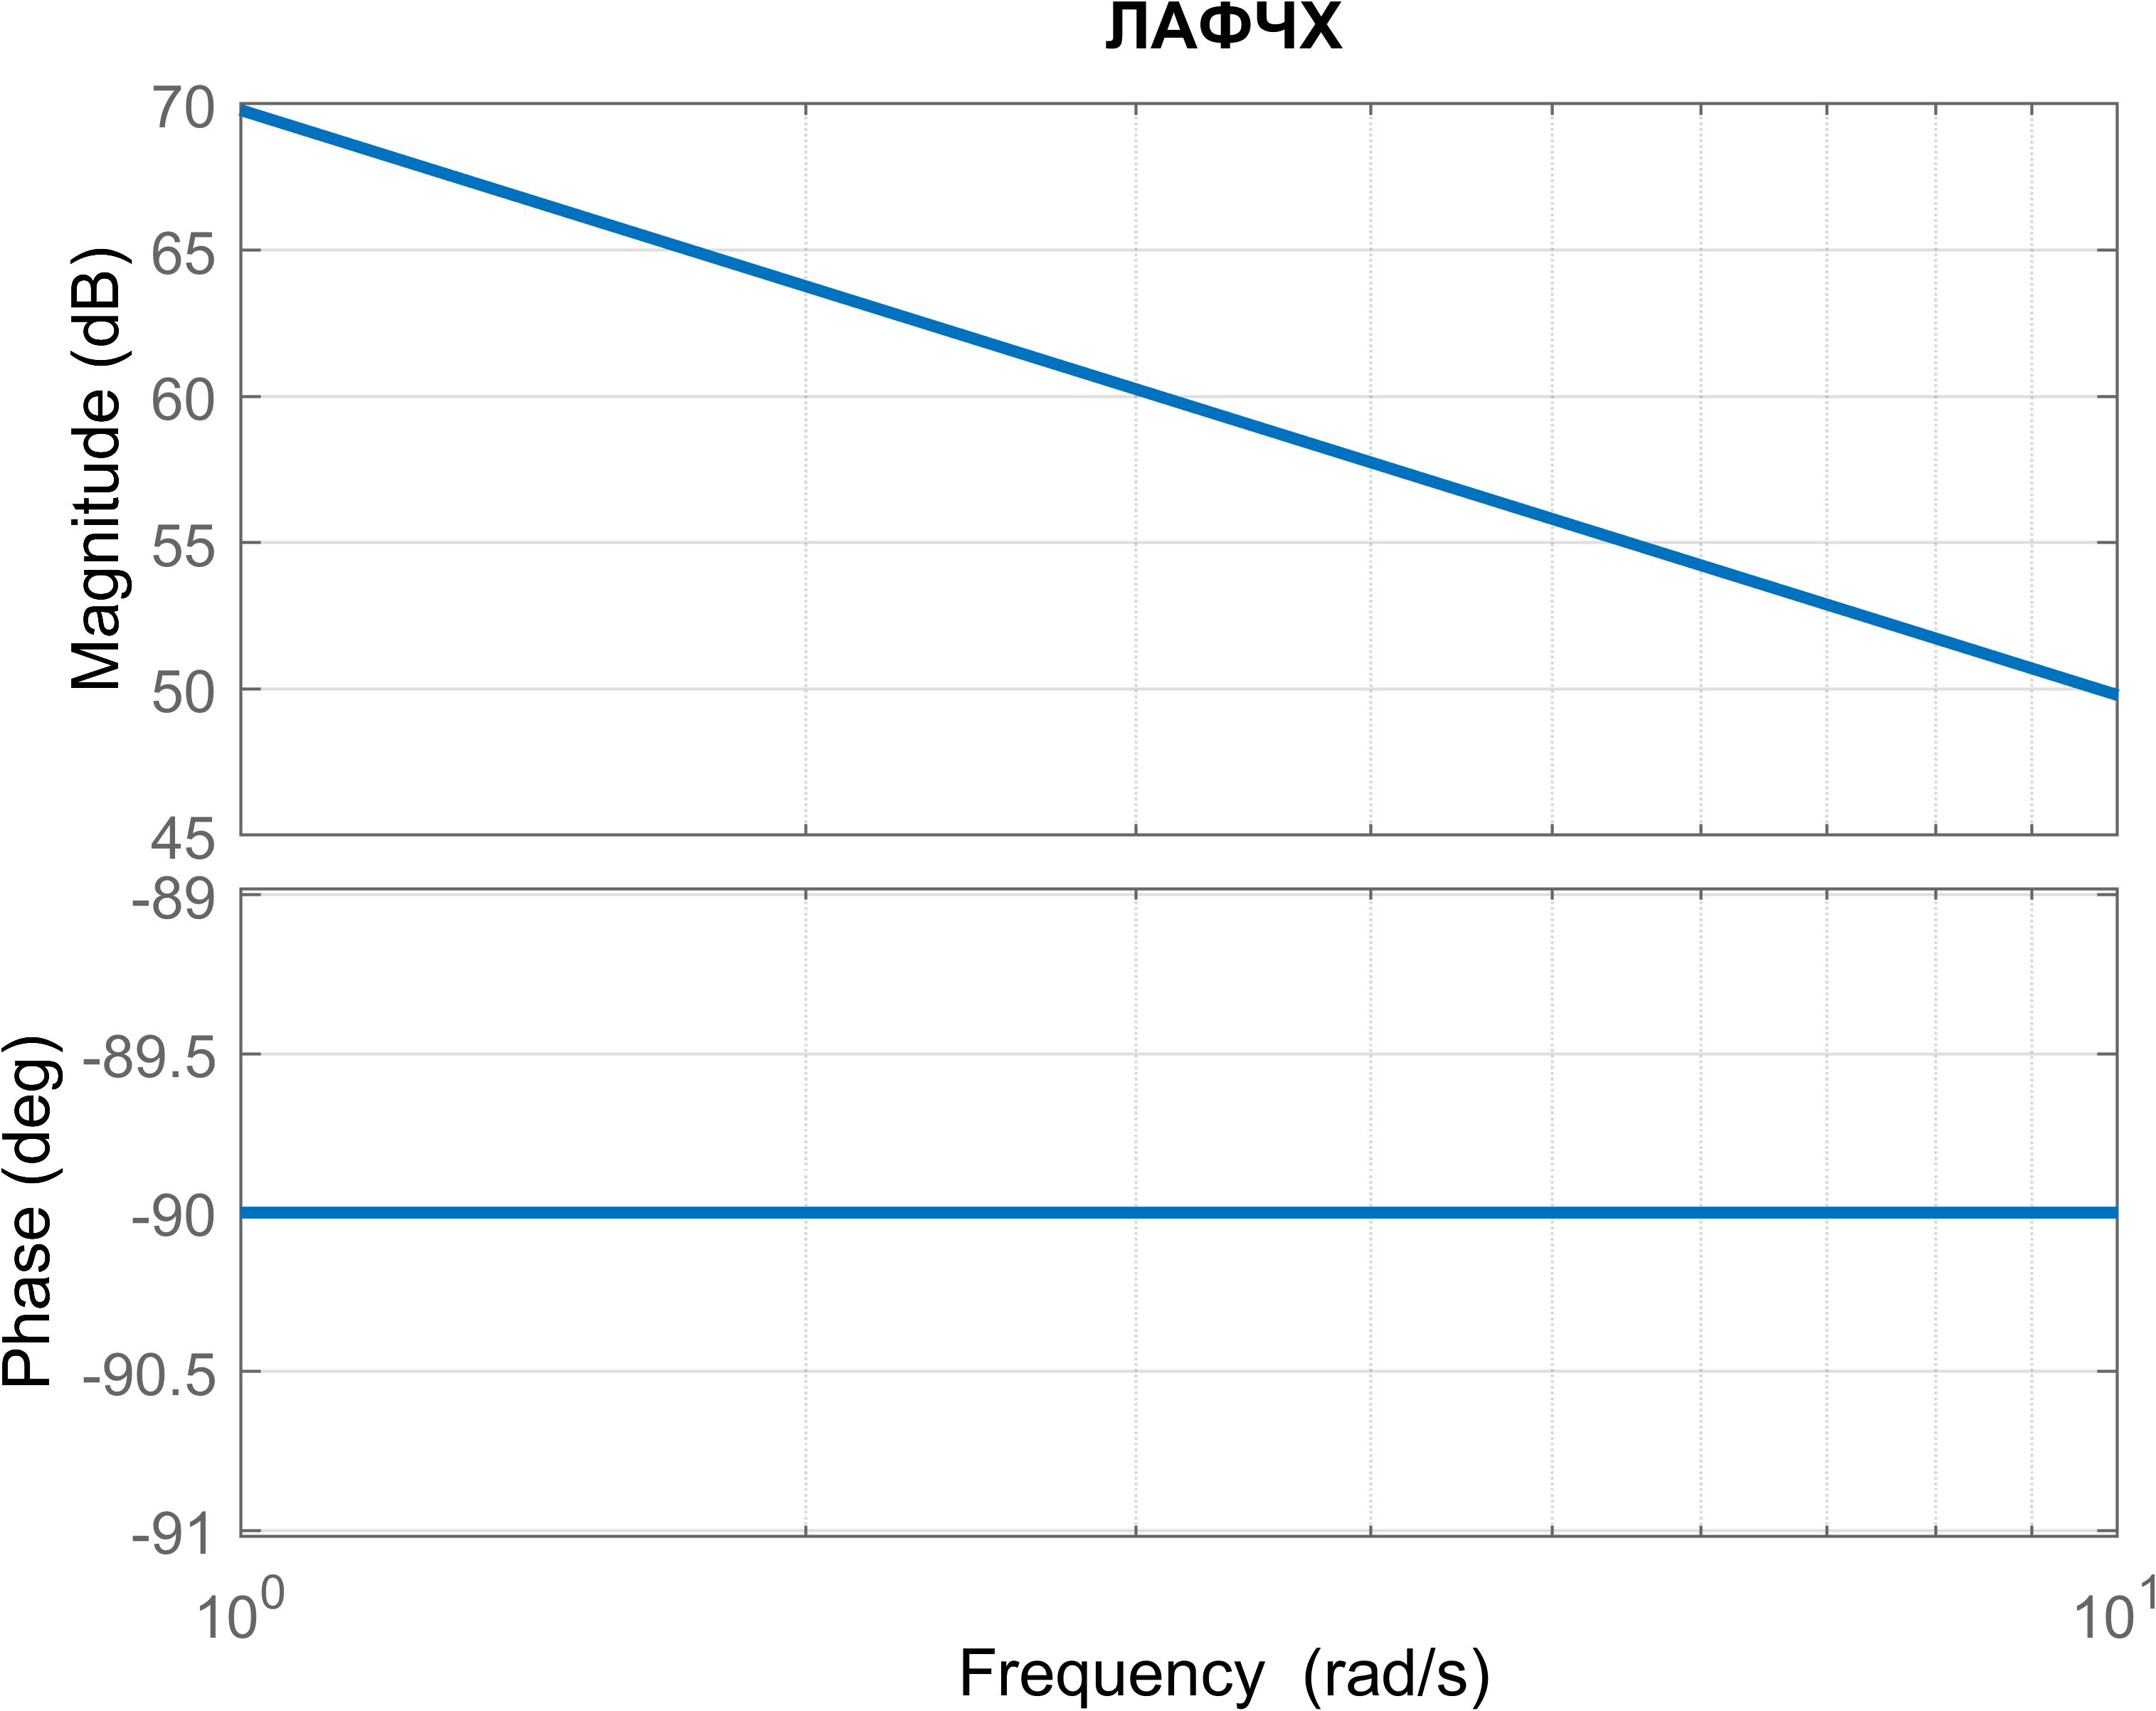
\includegraphics[width=0.75\textwidth, trim={0cm 0cm 0cm 0cm}]{../images/3_5.png}
    \caption{Логарифмическая амплитудно-фазо-частотная характеристика конденсатора}
\end{figure}
\endinput